% Author: Alexander Feng
% Emails: alexfeng2000@berkeley.edu
% Source: Prof. Vladimir Dobrushkin, http://www.cfm.brown.edu/people/dobrush/am33/Mathematica/ch2/pursuit.html
% Source: Molly Severdia, https://mse.redwoods.edu/darnold/math55/DEproj/sp08/mseverdia/pursuit.pdf


\iffalse
This problem was created as a neat application of differential equations and linearization.
\fi

\qns{Pursuit Curves}

In the following graphic, we see an example of a pursuit curve.
If you took CS61BL, you may recall this curve from one of the first labs.

\begin{center}
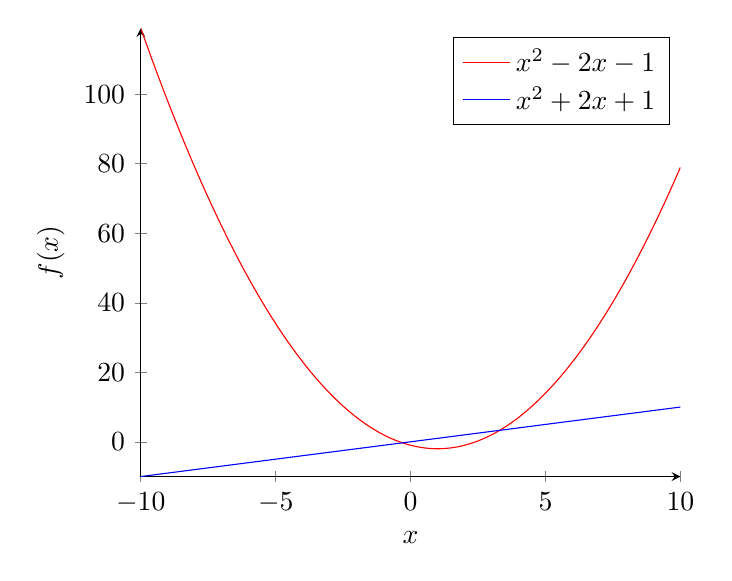
\begin{tikzpicture}
\begin{axis}[
    axis lines = left,
    xlabel = $x$,
    ylabel = {$f(x)$},
]
%Below the red parabola is defined
\addplot [
    domain=-10:10,
    samples=100,
    color=red,
]
{x^2 - 2*x - 1};
\addlegendentry{$x^2 - 2x - 1$}
%Here the blue parabloa is defined
\addplot [
    domain=-10:10,
    samples=100,
    color=blue,
    ]
    {x};
\addlegendentry{$x^2 + 2x + 1$}


\end{axis}
\end{tikzpicture}
\end{center}

The idea is simple, given a prey $P$, we would like to draw the curve of the predator $PR$ where the predator is pursuing $P$ such that $PR$ is always directly running at $P$.
However, the ratio of their velocities always remains a constant $K$.

\begin{enumerate}

\qitem Provided the velocities $\vec{V}_{P}$ and $\vec{V}_{PR}$, the positions $P$ and $PR$, write out a system of vector differential equations that describes this relationship in any number of dimensions.

\sol{
We can model this scenario with the following set of equations.
First, we know that the ratio of their velocities are always constant.
We also know that because $PR$ runs directly at $P$, the unit vector described by $P - PR$ is the same as the unit vector describing the velocity of $PR$.
This is because velocity is just magnitude and direction.
Thus, we get the following:

\begin{gather*}
K = \frac{\left\lVert\vec{V}_{PR}\right\rVert}{\left\lVert\vec{V}_{P}\right\rVert} \\
\frac{\vec{V}_{PR}}{\left\lVert \vec{V}_{PR} \right\rVert} = \frac{P - PR}{\left\lVert P - PR \right\rVert}
\end{gather*}


Substituting one into the other, we the following:

\begin{align*}
\vec{V}_{PR} = K \left\lVert \vec{V}_{p} \right\rVert \frac{P - PR}{\left\lVert P - PR \right\rVert}
\end{align*}

}



\end{enumerate}
